\hypertarget{les-uxeeles-sous-le-vent-uxe7a-secoue}{%
\section{Les Îles-Sous-Le-Vent, ça secoue
!}\label{les-uxeeles-sous-le-vent-uxe7a-secoue}}

\emph{Lundi 20 août 2018}

Comme on nous l'a dit pendant une excursion en bateau, les Polynésiens
ne le sont pas pour rien : nous avons constaté pendant la suite de notre
séjour toute l'étendue de leur polyvalence, et celle de leurs îles. Tour
d'horizon de ce que nous avons vu et fait dans les Îles-sous-le-vent.
Pour ceux qui ne sont pas familiers du terme, l'archipel où nous avons
voyagé s'appelle l'archipel de la Société. Vers l'Est se trouvent Tahiti
et Moorea, les Îles-du-vent, et vers l'Ouest se trouvent principalement
Bora-Bora, Maupiti, Raiatea, Tahaa et Huahine. Hormis cette dernière (où
nous n'avons pas mis les pieds), nous avons arpenté ces îles en long, en
large et en travers !

\begin{figure}
\centering
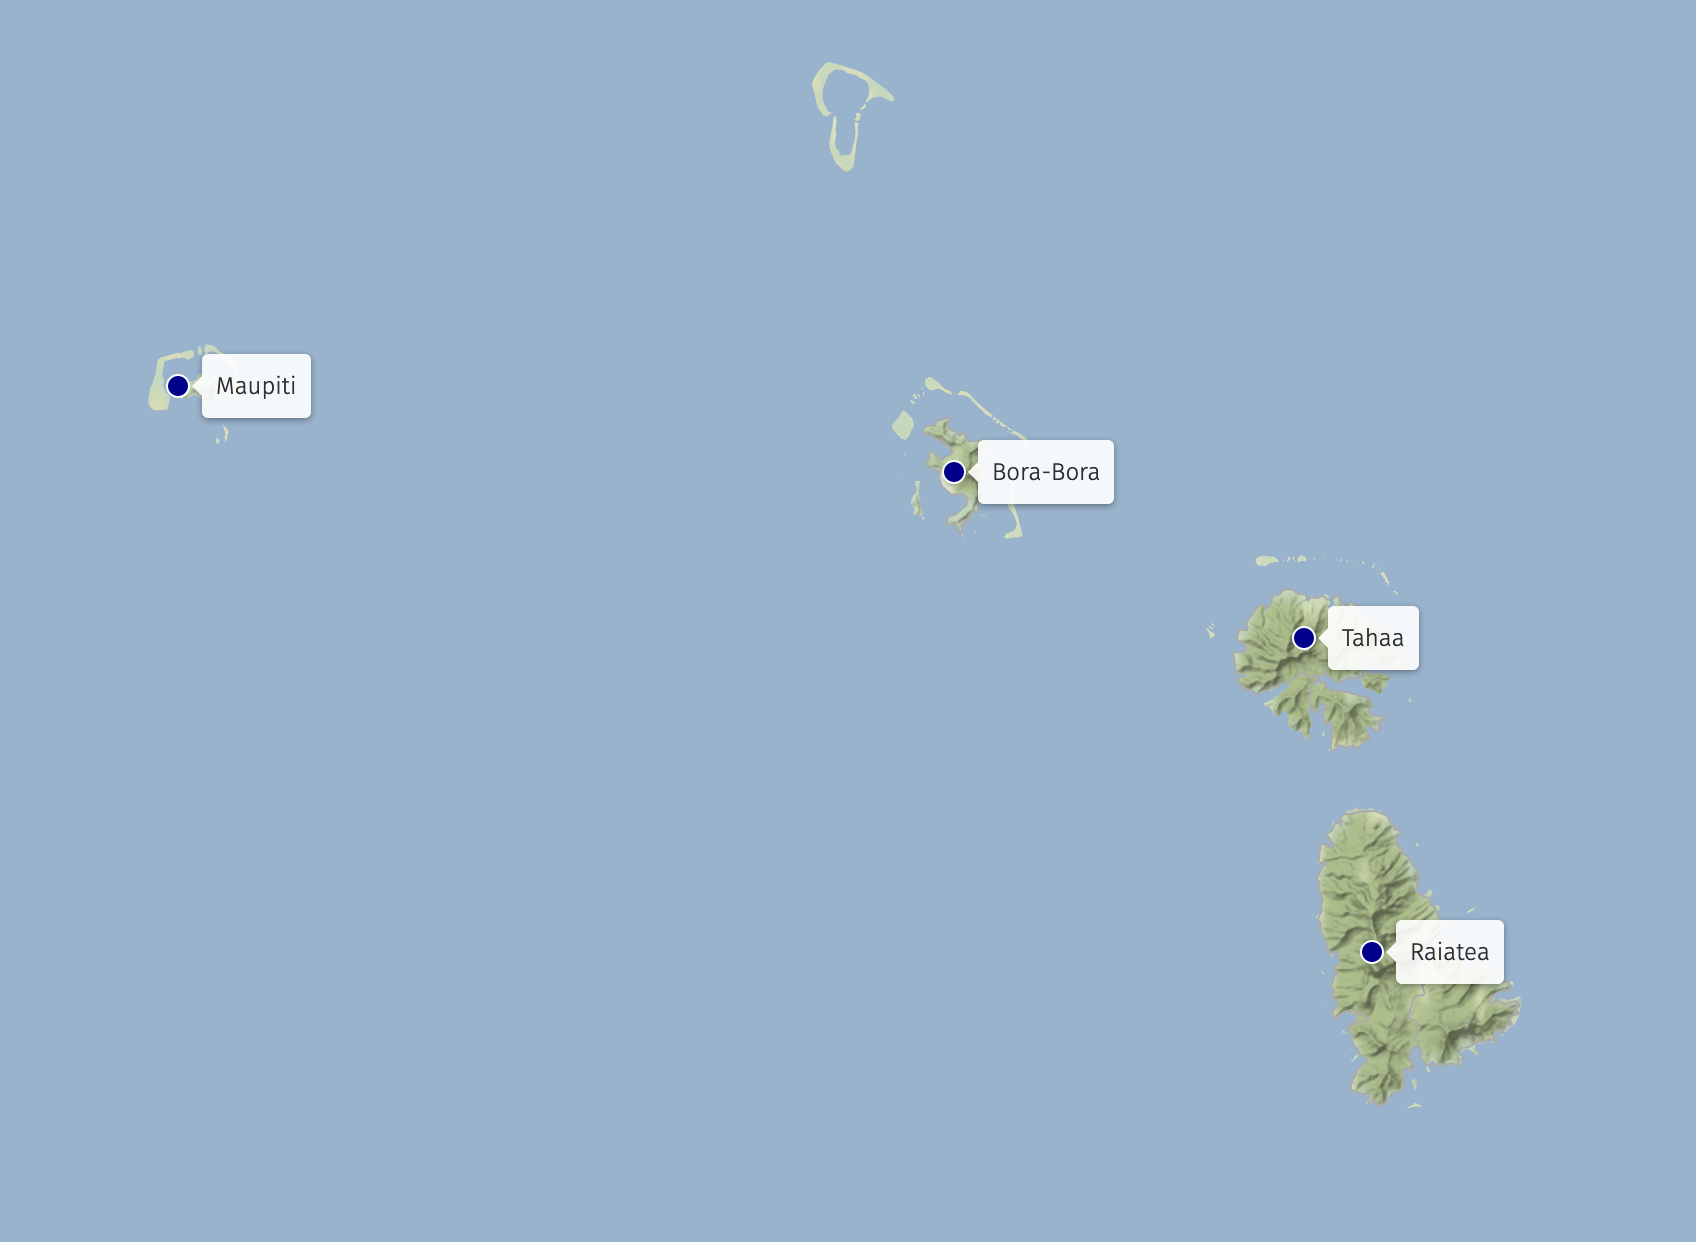
\includegraphics{maps/Polynesie2_1.png}
\caption{Arrivée à Bora-Bora et son lagon sublime !}
\end{figure}

Attention, long article en vue mais on vous met plein de photos, on a eu
du mal à choisir !

\hypertarget{bora-bora}{%
\subsection{Bora-Bora}\label{bora-bora}}

\begin{figure}
\centering
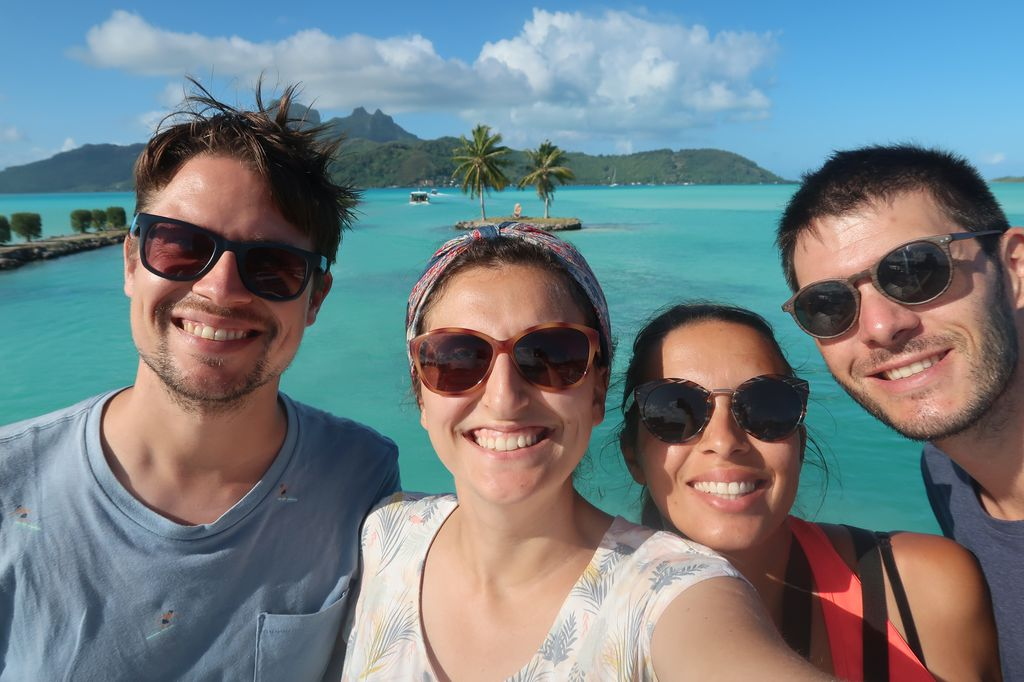
\includegraphics{images/20180820_boraselfie.JPG}
\caption{Arrivée à Bora-Bora et son lagon sublime !}
\end{figure}

Et nous avons commencé par Bora-Bora, dont le nom était porteur de plein
d'images de carte postale et aussi source d'inquiétudes. En effet, les
prix étant significativement plus élevés sur cette île, nous avions fait
le plein de courses à Tahiti (et même depuis l'Australie !). Ce qui
marque en premier quand on survole Bora, c'est la forme de ses
montagnes, très singulière. Ensuite, c'est pendant la traversée en
bateau pour rejoindre l'île principale depuis le motu (îlôt de sable) de
l'aéroport que le bleu du lagon nous impressionne : pour le coup on sait
qu'on y est, dans la carte postale !

Et puis Bora, c'est synonyme d'hôtels de luxe, avec les fameux bungalows
au-dessus de l'eau. On voit bien les bungalows quand on fait le tour du
lagon, mais on croise moins leurs locataires, qui doivent donc être
assez peu nombreux et sans doute cantonnés aux activités proposées par
leur hôtel. Ce qui fait qu'on a été agréablement surpris. On s'attendait
à se retrouver à Saint-Tropez et finalement on aura côtoyé surtout des
polynésiens ! Et tout particulièrement la famille qui nous a reçu tous
les quatre : l'accueil chaleureux et généreux de Mataha, JP et les
filles nous a fait nous sentir comme à la maison. On se souviendra
longtemps de Tiheni, 4 ans, qui joue au coiffeur avec les garçons : "tu
veux quoi comme coupe ? Bôgosse ?" :D

\begin{figure}
\centering
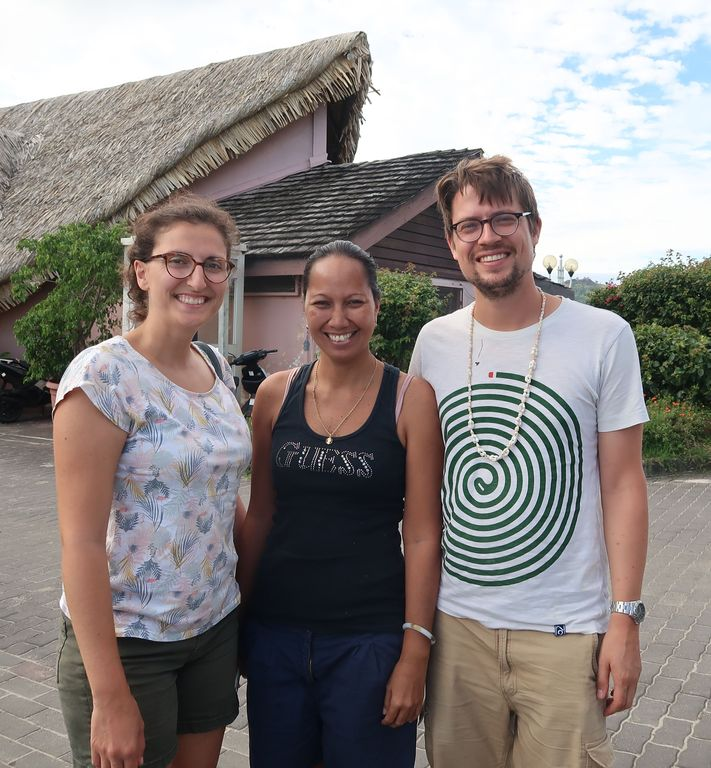
\includegraphics{images/20180820_mataha.JPG}
\caption{Notre hôte à Bora-Bora : Mataha (et sa famille).}
\end{figure}

Après une première journée à faire le tour de l'île en vélo (34 km),
histoire de mieux comprendre où on est (avec une flotte de vélos à un
disque et sans freins et un tricycle, je vous laisse imaginer la galère,
heureusement que c'est presque tout plat !), on a enchaîné le lendemain
avec le tour de l'île en bateau. Comment ne pas profiter du lagon, un
des plus beaux atouts de l'île : on a commencé par nager avec une
impressionnante raie manta, puis nous avons retrouvé nos copines les
raies pastenagues et les requins à pointe noire, puis une exploration du
jardin de corail avec ses bancs de poissons colorés et ses coquillages
presque fluorescents... Le tout entrecoupé d'un délicieux repas
polynésien, en phase avec la nature : plats et assiettes en feuilles de
bananier tressées, "Les fourchettes ? Vos doigts. Les couteaux ? Vos
dents !".

Pendant une journée pluvieuse, on s'est baladés avec JP qui nous a
raconté plein de choses, dont l'utilisation du noni, un fruit qui sent
vraiment très mauvais, exporté aux Etats-Unis pour en faire des
jus-qui-guérissent-tout. On parle aussi de l'histoire des bunkers qui se
trouvent aux quatre coins de l'île (aujourd'hui encore utilisés comme
refuge en cas de cyclone), construits par les américains pendant la
seconde Guerre Mondiale après l'attaque de Pearl Harbor. Ils ont utilisé
Bora comme base et y ont construit le premier aéroport de Polynésie.

On s'est aussi lancés dans une activité peu pratiquée à Bora : la
randonnée. L'ascension du Mont Ohue, à plus de 660 mètres d'altitude,
nous a donné bien du fil à retordre. 3 heures de montée, autant de
descente, un balisage au scotch gris dans les arbres, des passages avec
des cordes et le tout sur un terrain glissant au vu des pluies de la
veille...et on oublie toutes les peines une fois arrivés en haut : la
vue est à couper le souffle (et non, c'est pas que à cause de la fatigue
!), on a du mal à vouloir redescendre. D'ailleurs, on paiera nos
exploits pendant 3 jours avec de bonnes courbatures, qu'on traînera
jusqu'à l'île suivante : Maupiti !

\begin{figure}
\centering
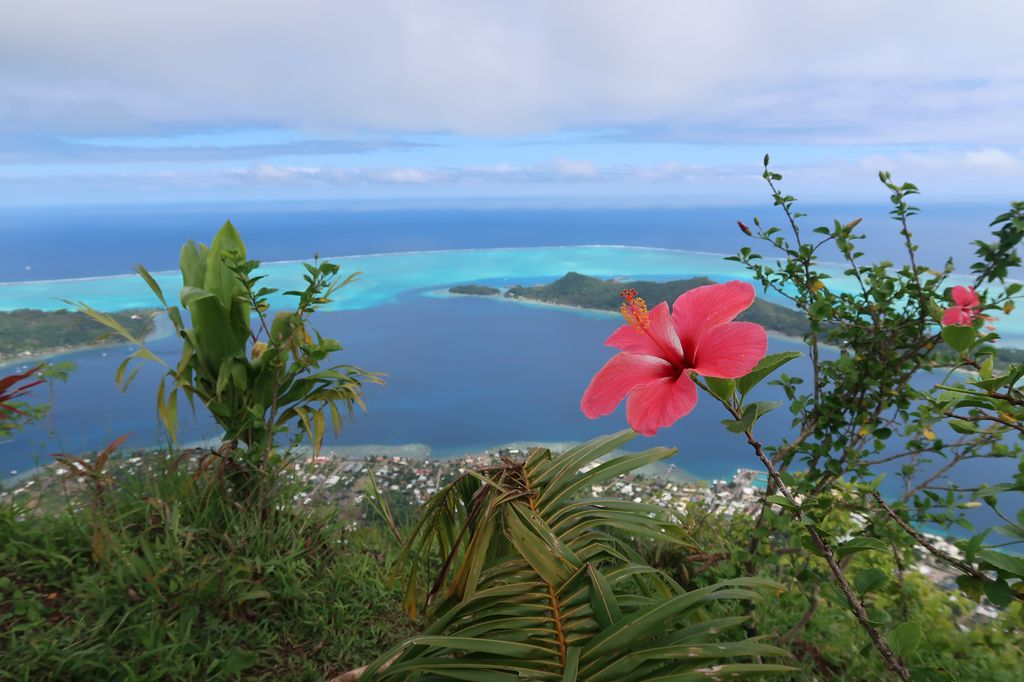
\includegraphics{images/20180820_borarando.JPG}
\caption{La vue depuis le sommet de Bora-Bora !}
\end{figure}

\hypertarget{maupiti}{%
\subsection{Maupiti}\label{maupiti}}

Maupiti a un charme bien à elle, et très différent de Bora. A commencer
par sa taille : 10 kilomètres de circonférence, un petit millier
d'habitants, qui ont voté par référendum l'interdiction des hôtels sur
l'île. Ils gèrent donc le tourisme sur leur île avec plein de pensions
de famille et chacun son bateau pour emmener les locataires en
excursion. C'est d'abord chez Phirmin et Rose, puis chez leur neveu Ludo
que nous avons séjourné, échangé (des histoires et des chansons), et
dégusté de délicieuses spécialités locales ! On mange d'ailleurs
principalement les fruits et légumes qui poussent sur l'île, les
poissons du lagon et les poulets qui se baladent partout (on vous a pas
raconté encore les coqs qui crient à toute heure du jour et de la
nuit?). Quand on sait que le bateau de ravitaillement des quelques
magasins et des livraisons de commandes diverses et variées passe une
fois par mois, on comprend mieux l'intérêt d'une nature généreuse !

\begin{figure}
\centering
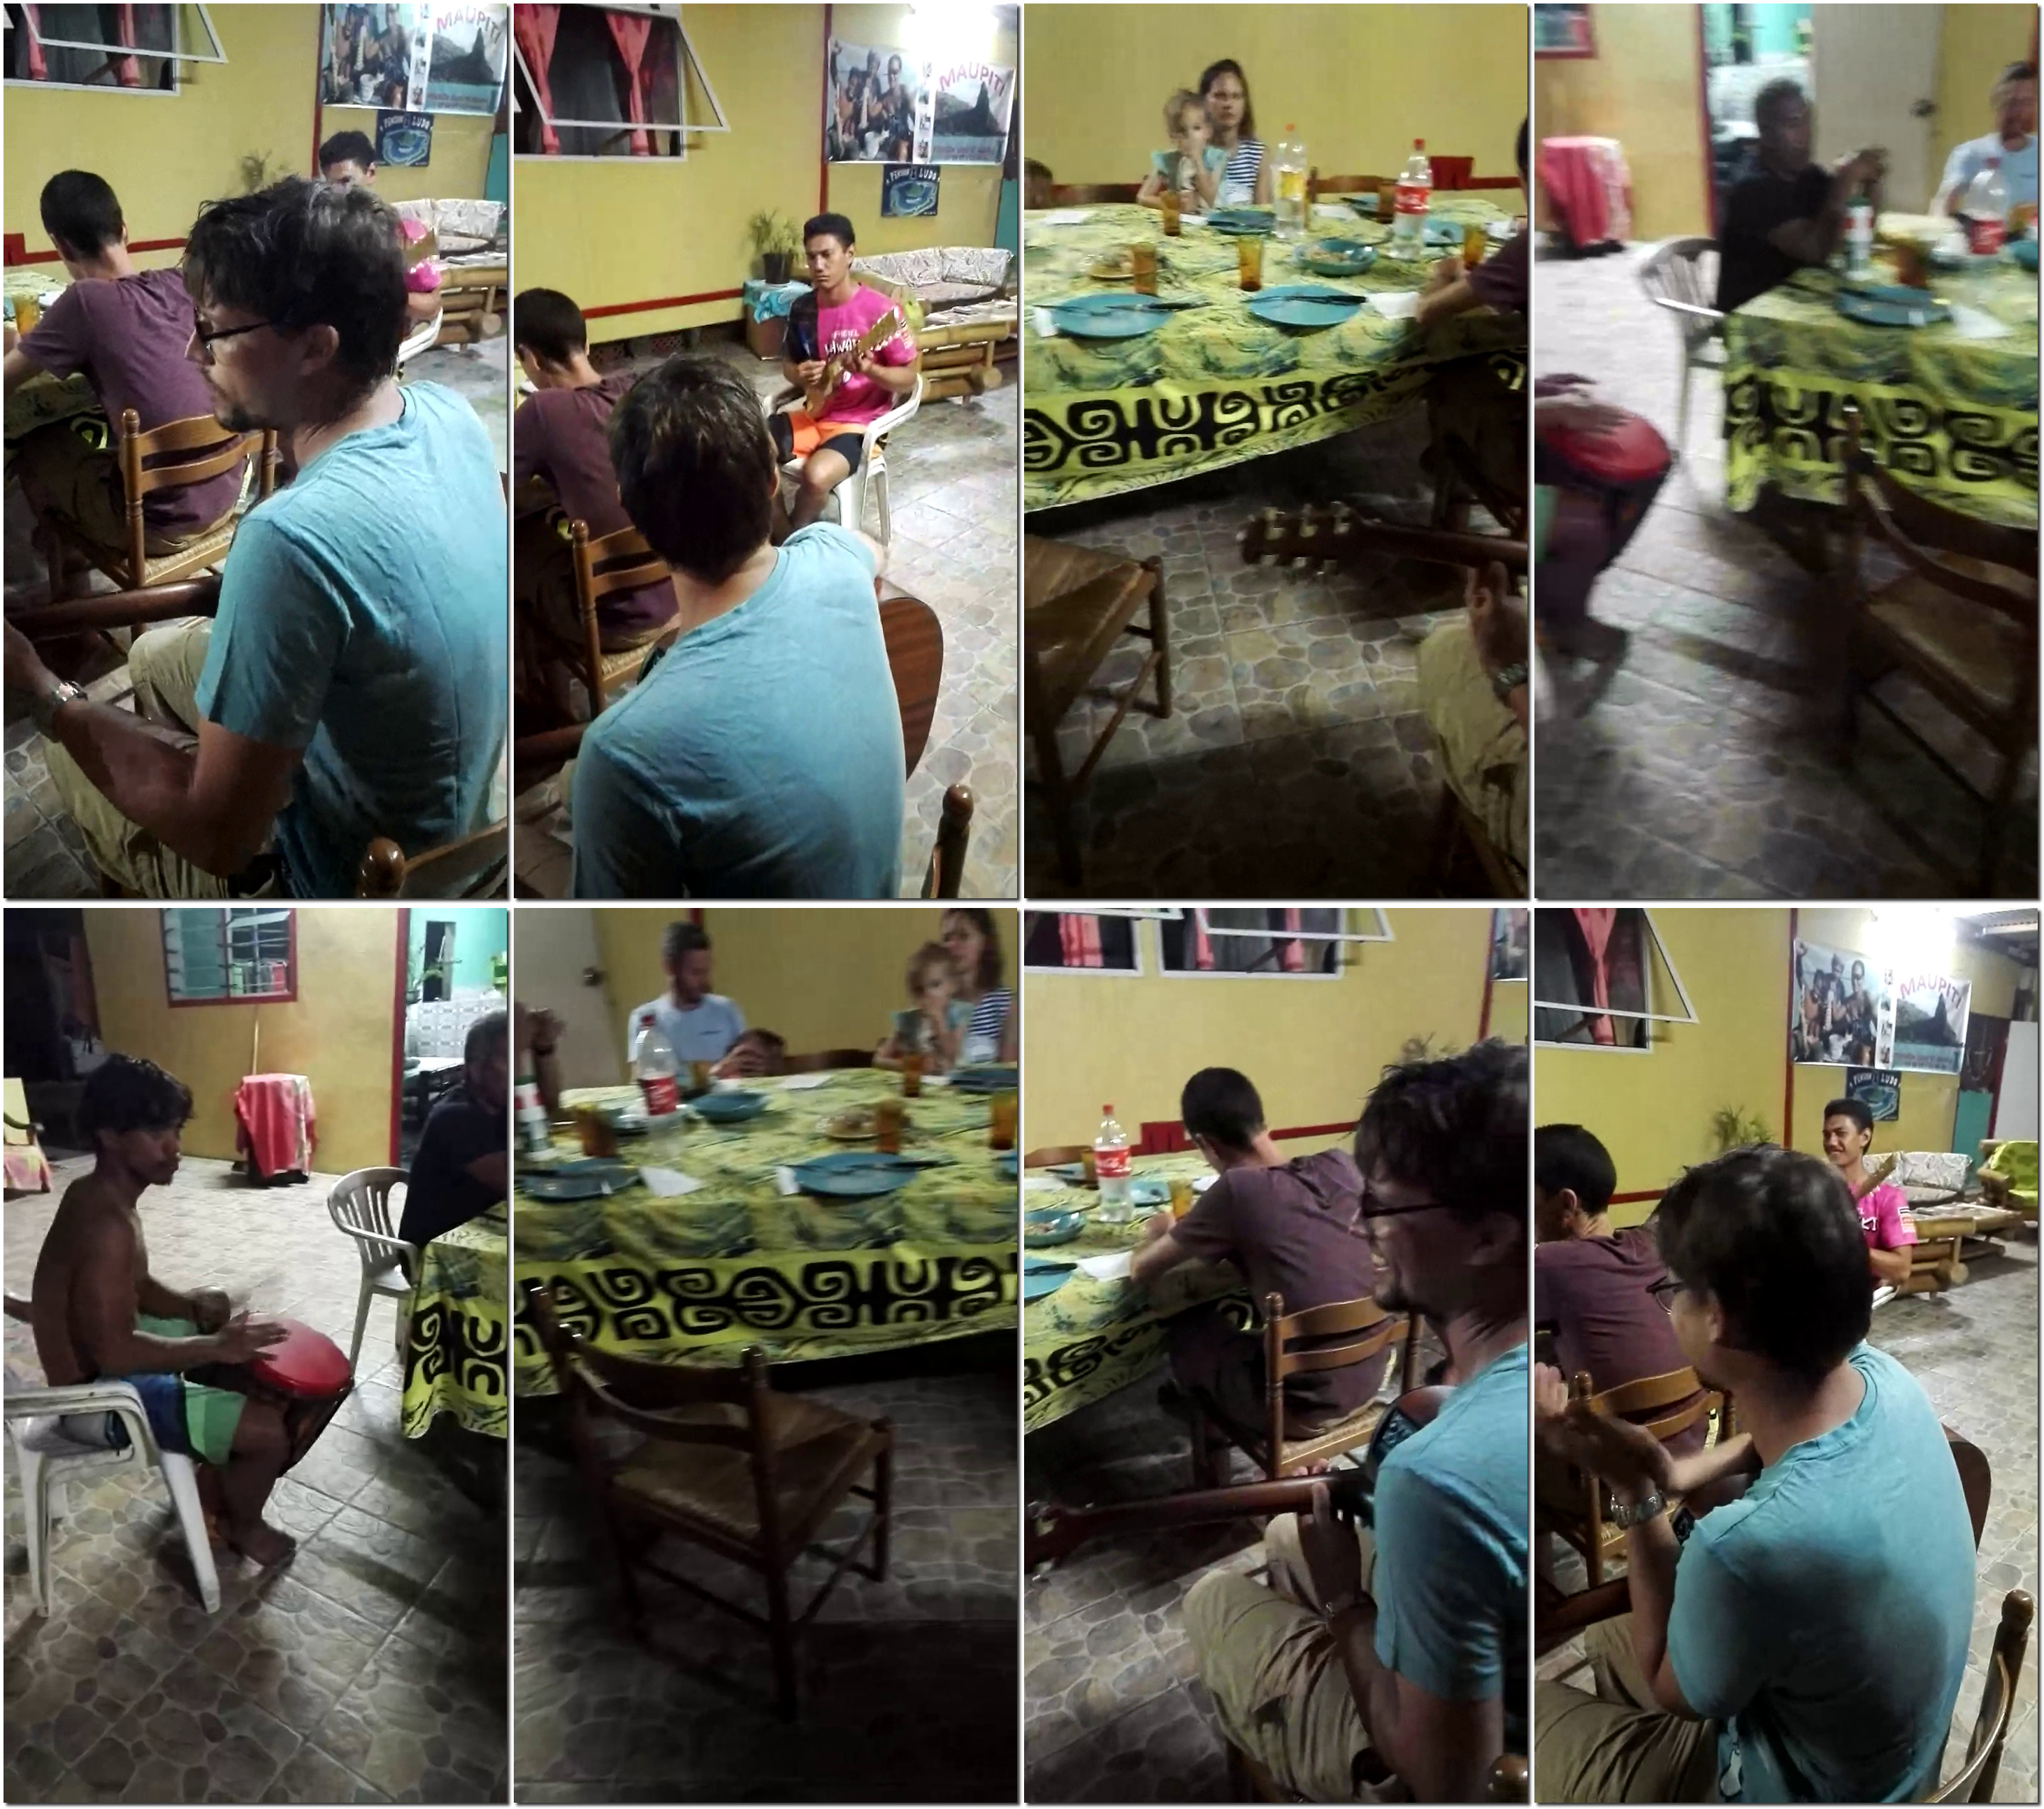
\includegraphics{montage/polynesie.jpg}
\end{figure}

Parmi nos ativités sur Maupiti, on est allés voir les raies manta, qui
nous ont offert un défilé sous le bateau (7 raies à la suite !) puis qui
se sont laissées admirer pendant qu'on se baignait à côté ; on a
découvert le jardin de corail (avec beaucoup moins de profondeur que
celui de Bora, on en a gardé quelques écorchures...), on a aussi fait le
tour de l'île à vélo (qui est bizarrement passé très vite \^{}\^{}), et
on a lézardé sur la plage (et l'unique) de la pointe Tereia. En face de
la plage se trouve un motu où étaient logés Camille et Guillaume,
accessible par une traversée de 20 minutes à pied sur le banc de sable,
avec de l'eau jusqu'à la taille. On y a passé une après-midi mémorable,
à jouer à un jeu de société et à se voir offrir des langoustes (qui ont
été plus ou moins délicatement explosées au penou, outil en pierre bien
pratique), pastèques et coco fraîches par Gilbert, le propriétaire. Le
pied !

\begin{figure}
\centering
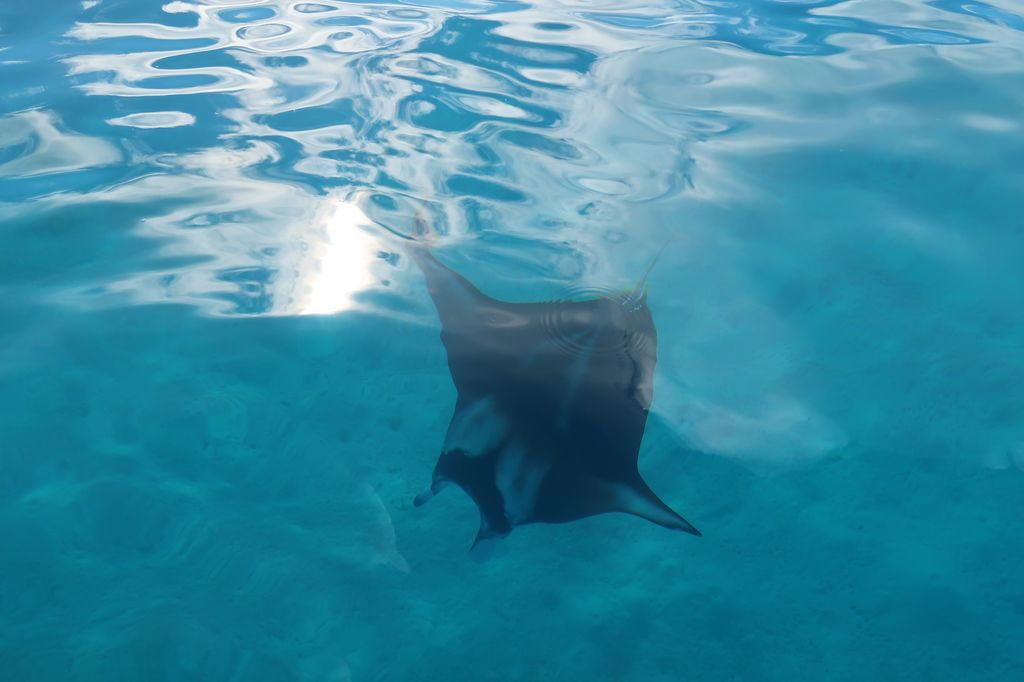
\includegraphics{images/20180820_raiemanta.JPG}
\caption{L'eau est tellement claire qu'on voit les raies manta depuis le
bateau.}
\end{figure}

Après deux jours de pluie on a finalement pu profiter d'une accalmie
pour se lancer dans l'ascension du Mont Teurafaatiu, qui nous a semblé
presque facile après celle de Bora ! Arrivés en haut dans un brouillard
épais, notre patience a fini par payer lorsqu'après de longues minutes
les nuages se sont dispersés, laissant apparaître progressivement une
vue magnifique à 280 degrés, qui n'a rien à envier à celle de la
randonnée précédente.

\begin{figure}
\centering
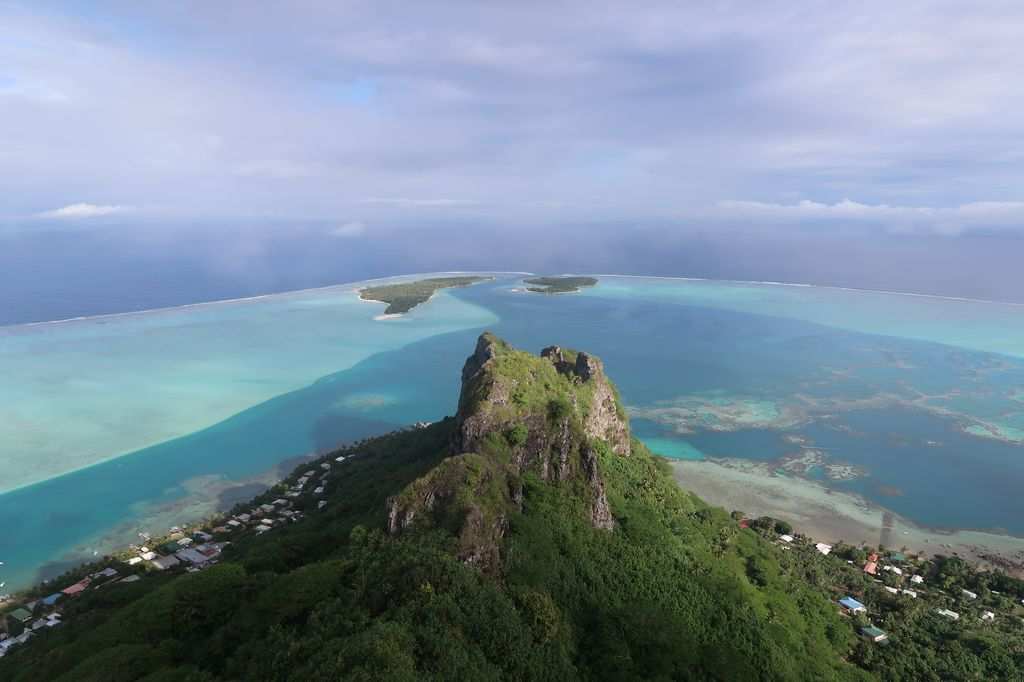
\includegraphics{images/20180820_maupitisommet.JPG}
\caption{Au sommet de Maupiti !}
\end{figure}

Et pour continuer dans le \emph{mana}, le départ vers l'aéroport en
bateau sous la pluie au lever du jour, avec plein de petits bateaux qui
affluent de tous les côtés pour emmener tout le monde vers le départ
avait un air irréel... Comme le dit la chanson qu'on nous a apprise ici
:

\begin{quote}
C'est une île bordée de bleu, une île bénie des dieux

Le ciel et la terre se marient, chaque jour, chaque nuit
\end{quote}

\hypertarget{raiatea}{%
\subsection{Raiatea}\label{raiatea}}

C'est sur Raiatea que nous avons passé les derniers jours dans les îles
de la Société. Ça a aussi été l'occasion de nous essayer au
Couchsurfing, et on n'a pas été déçus : l'accueil trois étoiles que nous
a réservé Justine, une kiné Lilloise qui a quitté le continent depuis
plusieurs années maintenant, était juste parfait pour notre fin de
séjour. L'île est un peu plus grande que la précédente, avec un bon 100
kilomètres de circonférence qu'on a découvert en voiture, en s'arrêtant
au grand \emph{marae} de Taputapuatea, site archéologique où se
rassemblaient des chefs de toutes les îles alentour, jusqu'à Hawaï.

On ne pouvait pas passer par Raiatea sans découvrir sa petite sœur,
Tahaa l'île vanille, qui partage le même lagon. C'est avec Yvann et son
beau-fils qu'on a passé une belle journée, du tour du lagon avec
exploration du jardin de corail, à la ferme perlière où on a découvert
les techniques légèrement barbares du processus pour obtenir les
fameuses perles noires de Tahiti. Après un poisson sauce vanille à
tomber (où seuls les regards pressants du reste de la tablée nous ont
fait lâcher le plat plein de sauce), on est passés par la coopérative de
la Vallée de la Vanille, dont l'exploitation a été lancée pour la
réinsertion professionnelle des habitants de l'île qui ont travaillé
dans les essais nucléaires français de la région. Le retour au coucher
de soleil au son des ukulélés sur le bateau était une belle conclusion à
l'excursion...

\begin{figure}
\centering
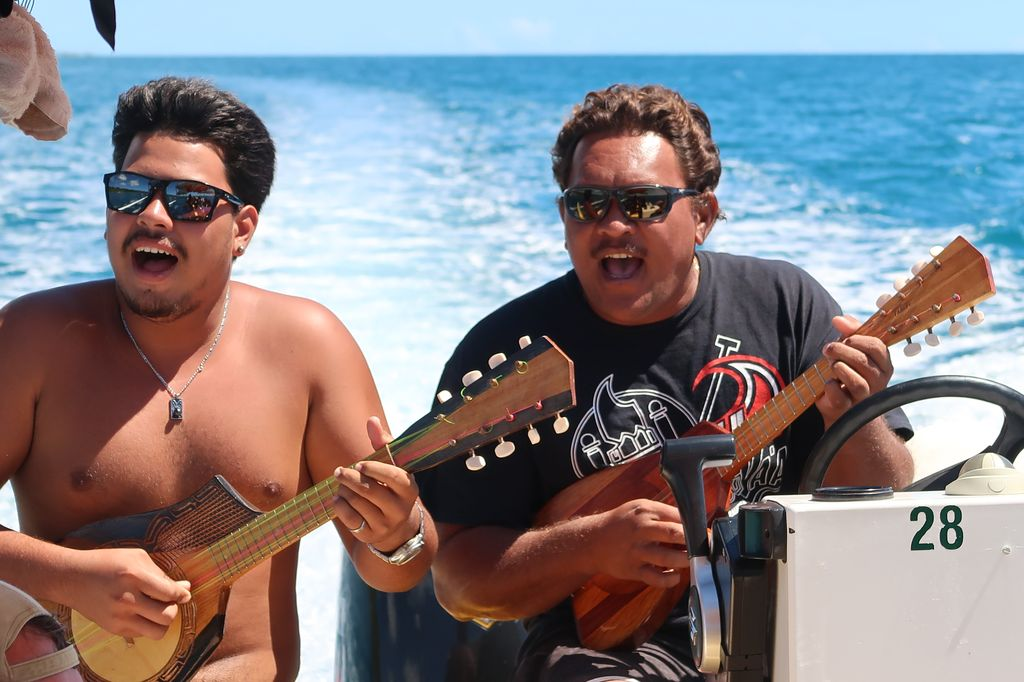
\includegraphics{images/20180820_tahaa.JPG}
\caption{Quoi de plus agréable qu'une excursion en bateau avec de la
musique ?}
\end{figure}

Pour dire au-revoir aux îles, il n'y avait rien de mieux que la
randonnée du mont Tapioi, au-dessus de la ville d'Uturoa, d'où on
pouvait voir aussi bien Bora-Bora, que Tahaa et Huahine (que nous
n'avons pas eu la chance et le temps de découvrir...). C'est avec un
pincement au cœur qu'on est redescendus de la montagne, mais Flo a
acquis un objet qui restera chargé de beaux souvenirs, et que les plus
chanceux d'entre-vous auront l'occasion de découvrir, voire même
d'entendre ;) A l'aéroport, en entendant un émouvant chant d'au-revoir
d'une famille polynésienne qui se séparait, c'est les larmes aux yeux
qu'on embarque dans l'avion.

\begin{figure}
\centering
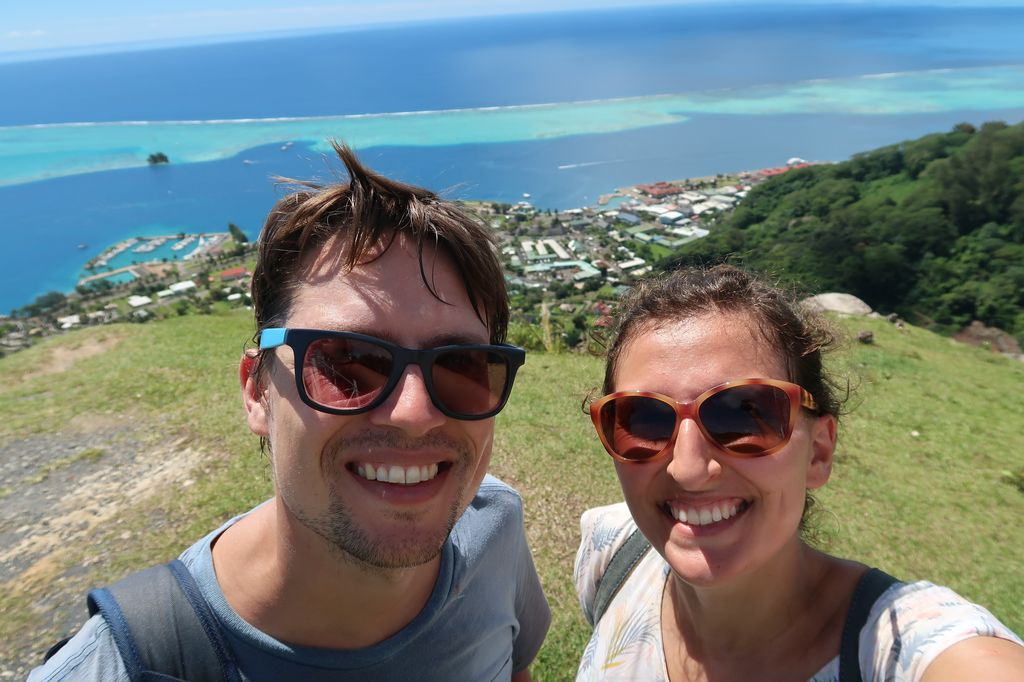
\includegraphics{images/20180820_raiatea.JPG}
\caption{Nos adieux (joyeux) depuis le mont Tapioi.}
\end{figure}

Après ces semaines en Polynésie, on comprend pourquoi tant de monde
tombe amoureux de ces îles : on n'en revient pas indemne. D'ailleurs,
Justine nous a présenté une joyeuse bande de métropolitains, aux
histoires toutes plus incroyables et improbables les unes que les
autres, mais qui finissent toujours pareil : "et puis, je suis arrivé
ici, et je suis jamais reparti...".

\hypertarget{bonus}{%
\subsection{Bonus}\label{bonus}}

\hypertarget{quizz-des-uxeeles}{%
\subsubsection{Quizz des îles}\label{quizz-des-uxeeles}}

Voici un certain nombre de questions collectionnées au fur et à mesure
des trois semaines en Polynésie qui nous ont tenu en haleine jusqu'aux
derniers jours.

\begin{itemize}
\tightlist
\item
  pourquoi suspend-t-on les bateaux \emph{au-dessus} de l'eau ? Pour les
  protéger des huîtres qui mangent le bois des bateaux (même si
  aujourd'hui on n'en a plus vraiment besoin avec les nouvelles
  peintures) !
\item
  que veut dire le signe suivant et d'où vient-il ? Le signe signifie
  hang-loose et vient des surfeurs Hawaïen (y'a même une petit légende
  associée).
\end{itemize}

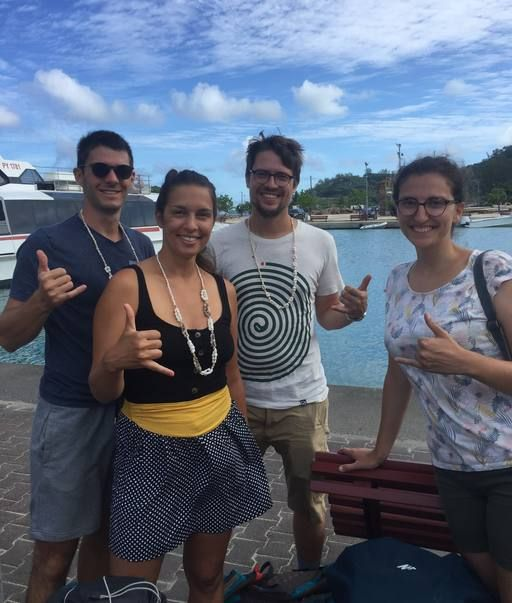
\includegraphics{images/20180820_hangloose.jpg}

\begin{itemize}
\tightlist
\item
  c'est quoi être \emph{fiu} ? C'est quand on en a marre et qu'on ne
  travaillera plus de la journée !
\item
  quand on entend un gros boum, c'est quoi ? La coco qui vient de tomber
  du palmier !
\item
  c'est quoi un motu (prononcer motou) ? Ce sont les petites îles de
  sable que l'on voit un peu partout autour de l'île principale.
\item
  à qui appartiennent les poulets qu'on voit partout ? A tout le monde
  (et la légende dit qu'on peut les manger) !
\item
  c'est quoi le coprah ? De la noix de coco qu'on fait sécher dans des
  hangars à toits ouvrants un peu partout sur les îles. On livre le tout
  par sac de 25 kilos à l'usine de Tahiti quand le bateau cargo passe.
  Ca devient in-fine du monoï, de l'huile...
\item
  qu'est-ce qui fait des trous au bord de la route et fuit à l'approche
  des vélos ? Les crabes du bord de route !
\end{itemize}

\hypertarget{bougainville-uxe0-tahiti}{%
\subsubsection{Bougainville à Tahiti}\label{bougainville-uxe0-tahiti}}

Une lecture historique sur la visite du navigateur Bougainville à Tahiti
en 1768, disponible sur Gallica. Pour les curieux des premières
descriptions de Tahiti en VO.

\hypertarget{le-chant-des-baleines}{%
\subsubsection{Le chant des baleines}\label{le-chant-des-baleines}}

Grâce à la caméra GoPro de Camille et Guillaume, nous avons le plaisir
de partager avec vous un extrait du chant des baleines lors de notre
sortie snorkelling à Moorea :

\emph{Elida et Florian}
